% !TEX root = ../Dokumentation.tex
\subsection{Chassis}

\textbf{Funktionsbeschrieb}
\\[0.2cm]
Im Lösungskonzept wird ein Chassis mit vier Rädern verwendet. Die Hinterräder werden mit einem DC-Getriebemotor angetrieben. Der Motor ist über ein Differentialgetriebe mit der Hinterachse verbunden. Das Differentialgetriebe erlaubt den beiden Hinterrädern in der Kurve unterschiedlich schnell zu drehen. Die Vorderräder sind frei drehbar. Der Achsabstand soll ein Mass von 160mm nicht überschreiten.\\
Für die Lenkung wird eine Achsschenkellenkung verwendet. Diese wird mittels einem Servomotor angetrieben. Wegen dem maximalen Achsabstand von 160mm ist der Servomotor zum Antrieb der Lenkung vor dem Fahrzeug verbaut.
\begin{figure}[H]%Position festigen
\centering
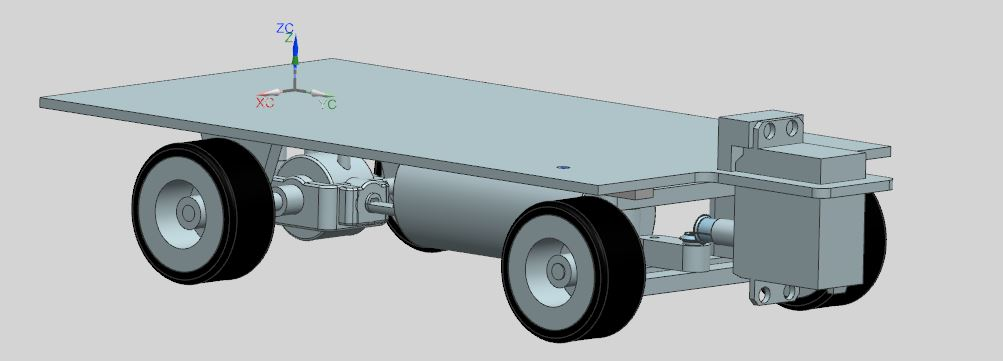
\includegraphics[width=1\textwidth]{03_Loesungskonzept/pictures/Chassis_2.JPG}
\caption{Konzept des Chassis}
\label{fig:activityRoute}
\end{figure}\flshleft
\textbf{Komponentenbeschrieb}
\\[0.2cm]
Der Antriebsmotor, ist ein 12 V Getriebemotor mit einer Getriebeuntersetzung von 1:18. Er hat somit eine Lastdrehzahl von 317 U/min. Zusammen mit der 2:1 Untersetzung des Differentialgetriebes, drehen die Hinterräder mit Durchmesser 43mm mit 158 U/min. Somit ist die maximale Geschwindigkeit des Fahrzeuges bei 35 cm/s.\\
Das Differentialgetriebe vom dem Modellbauhersteller Relly.
\begin{figure}[H]%Position festigen
\centering
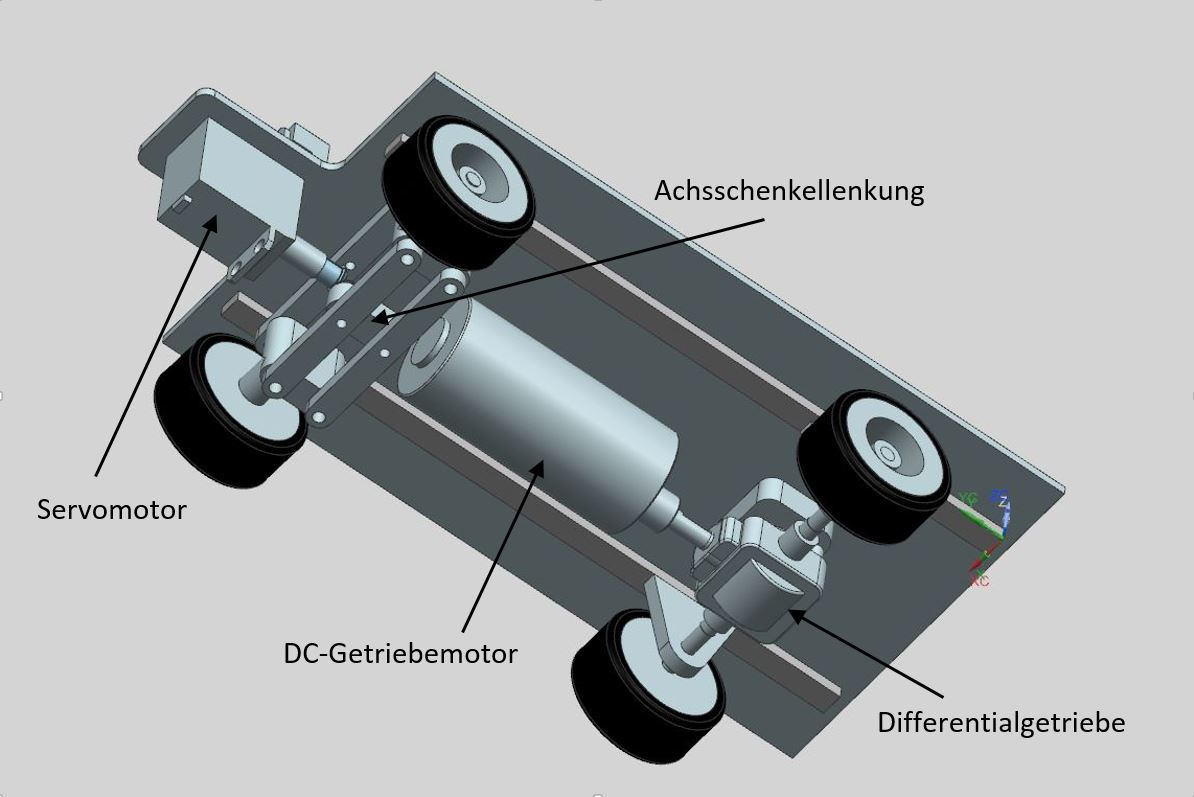
\includegraphics[width=1\textwidth]{03_Loesungskonzept/pictures/Chassis_1.JPG}
\caption{Konzept des Chassis mit Komponentenbeschriftung}
\label{fig:activityRoute}
\end{figure}\flashleft
\textbf{Begründung}
\\[0.2cm]
Das Konzept mit 4 Räder, einem Antriebsmotor und einer Achsschenkellenkung, hat sich durchgesetzt, weil die Regelung für die Spurhaltung wesentlich ruhiger ist als mit zwei Angetriebenen Rädern. Des weiteren ist die Lenkung und der Antrieb klar getrennt. Beim Antriebsmotor kann man auf teure Schrittmotoren verzichten und die Geschwindigkeit der Räder muss nicht mit einem sehr genauen Encoder bestimmen werden.